\section{频响分析法}

系统对正弦输入信号的稳态响应称为频率响应。通过改变输入信号的频率,考察系统产生的响应,可以作为分析和设计控制系统的重要依据。

正弦传递函数就是把系统传递函数中的$s$用$j\omega$代替所得到的函数,其中$\omega$为频率,单位为$rad/s$。当用$circ/s$为单位测量频率时,频率用$f$来表示,$\omega=2\pi f$。

传递函数可以表示为相位与辐角的形式

\begin{equation*}
    G(j\omega)=Me^{j\phi}=M\phase{\phi}
\end{equation*}

稳定的线性定常系统在收到正弦信号的输入后,在稳态时将会输出一个和输入信号频率相同的正弦输出信号。然而输出的幅值和相位一般和输入信号存在差异,这由正弦传递函数决定。

\begin{align*}
    |G(j \omega)|&=\left|\frac{Y(j \omega)}{X(j \omega)}\right|\\ 
    \phase{G(j \omega)}&=\phase{\frac{Y(j \omega)}{X(j \omega)}}
\end{align*}

\subsection{伯德图}

伯德图有两幅图组成,一幅是正弦传递函数幅值的对数坐标图,另一幅是相角图。两幅图的横坐标都是频率的对数。

对数幅值的表达式为$20\log\left|G(j\omega)\right|$,所得到的单位是分贝$dB$。

用MATLAB绘制伯德图的命令是

\begin{lstlisting}
    bode(num,den)
    bode(sys)
    [mag,phase,w]=bode(num,den,w)
\end{lstlisting}

得到的伯德图如图\ref{22}所示。

\begin{figure}[!ht]
    \centering
    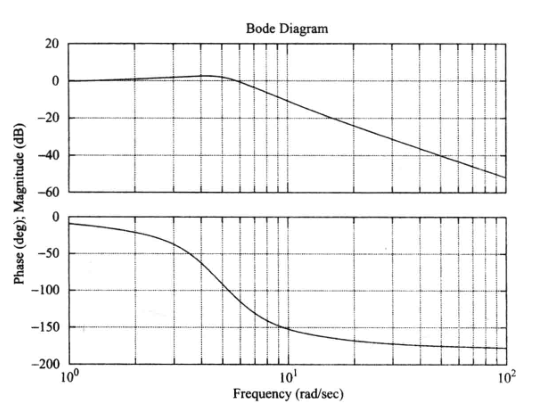
\includegraphics[width=8cm]{figures/22.png}
    \caption{伯德图}
    \label{22}
\end{figure}

\subsection{奈奎斯特图}

奈奎斯特图也称为极坐标图,是当$\omega$由零变到无穷大时,表示在极坐标上$G(j\omega)$的幅值和相角的关系图。如图\ref{23}所示。

\begin{figure}[!ht]
    \centering
    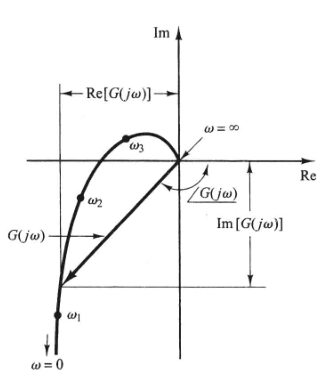
\includegraphics[width=8cm]{figures/23.png}
    \caption{奈奎斯特图}
    \label{23}
\end{figure}

用MATLAB绘制奈奎斯特图的命令是

\begin{lstlisting}
    nyquist(num,den)
    nyquist(sys)
    [re,im,w]=nyquist(num,den,w)
\end{lstlisting}

\subsection{奈奎斯特稳定判据}

\textbf{柯西辐角原理}

对于传递函数

\begin{equation*}
    \frac{C(s)}{R(s)}=\frac{G(s)}{1+G(s)H(s)}
\end{equation*}

系统稳定的条件为特征方程

\begin{equation*}
    1+G(s)H(s)=0
\end{equation*}

的根均位于$s$左半平面。

通过分析映射后的辐角,如图\ref{24}所示,不难得到结论:在$s$平面内封闭曲线顺时针包围$F(s)$的零点一次,则映射后的封闭曲线在$F(s)$平面内顺时针包围原点一次。

\begin{figure}[!ht]
    \centering
    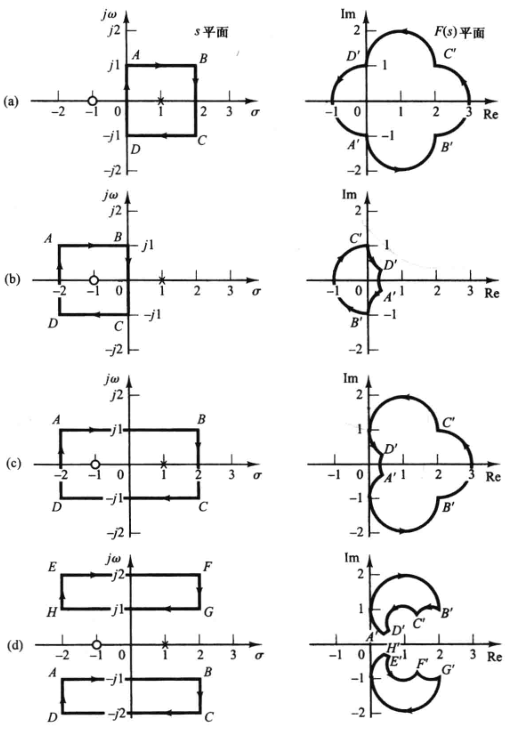
\includegraphics[width=8cm]{figures/24.png}
    \caption{$s$平面封闭曲线映射到$F(s)$平面的结果}
    \label{24}
\end{figure}

更一般地,则可以推广到柯西辐角原理:

\begin{equation*}
    N=Z-P
\end{equation*}

其中,$P$为$s$平面封闭曲线包围的$F(s)$极点数,$Z$为$s$平面封闭曲线包围的$F(s)$零点数,$N$为映射后$F(s)$平面封闭曲线顺时针包围原点的次数(若为负则代表逆时针包围)。

那么回到闭环传递函数与特征多项式

\begin{align*}
    T_0(s)&=\frac{C(s)G(s)}{1+C(s)G(s)}\\ 
    F(s)&=1+C(s)G(s)
\end{align*}

易得$F(s)$的零点,就对应着$T_0(s)$的极点。不妨假设$\Lambda_0(s)=C(s)G(s)$中分母的次数大于分子的次数,因此

\begin{equation*}
    \lim_{|s|\rightarrow\infty}F(s)=1
\end{equation*}

\begin{figure}[!ht]
    \centering
    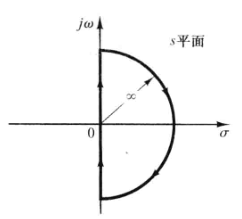
\includegraphics[width=8cm]{figures/25.png}
    \caption{$s$平面内封闭曲线的选取}
    \label{25}
\end{figure}

选取如图\ref{25}的封闭曲线,假设在虚轴上不存在零极点,则该曲线包围了右边平面$F(s)$全部的零极点。因此,如果我们知道了$\Lambda_0(s)$右半平面的极点数$P$,即可以通过观察$\Lambda_0(s)$奈奎斯特图中围绕点$(-1,j0)$点的次数$N$,就能得到$F(s)$的零点数$Z$。

因此,奈奎斯特稳定判据可以简单地表述为:如果开环传递函数$G(s)H(s)$在右半平面内有$P$个极点,则当$\omega$从$-\infty$变到$\infty$时,$G(j\omega)H(j\omega)$逆时针包围$(-1,j0)$点$P$次时,闭环系统稳定。

\subsection{$G(s)H(s)$含有位于虚轴上零极点的特殊情况}

当在虚轴上有开环传递函数的零极点时,就需要对$s$平面上的封闭曲线进行一定的改造,如图\ref{26}所示。

\begin{figure}[!ht]
    \centering
    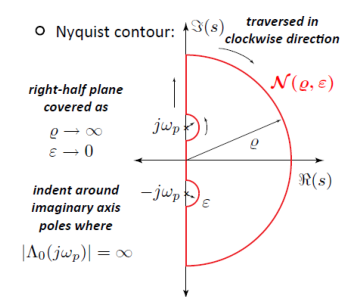
\includegraphics[width=8cm]{figures/26.png}
    \caption{$s$平面封闭曲线的改造}
    \label{26}
\end{figure}

例如:考虑开环传递函数

\begin{equation*}
    G(s)H(s)=\frac{K}{s(Ts+1)}
\end{equation*}

在$G(s)H(s)$平面上,对应$s=j0+$和$s=j0-$的点分别为$-j\infty$和$+j\infty$。在半径$\epsilon$的半圆轨迹上,如图\ref{27}所示,可以表示为

\begin{equation*}
    s=\epsilon e^{i\theta}\quad \theta=-90^\circ\rightarrow+90^\circ
\end{equation*}

\begin{figure}[!ht]
    \centering
    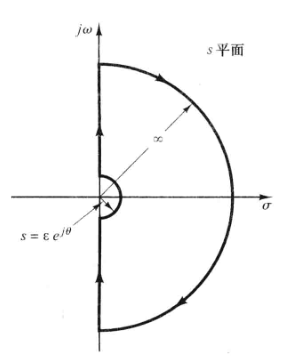
\includegraphics[width=8cm]{figures/27.png}
    \caption{改造后曲线}
    \label{27}
\end{figure}

对应的$G(s)H(s)$变为

\begin{equation*}
    G\left(\varepsilon \mathrm{e}^{j \theta}\right) H\left(\varepsilon \mathrm{e}^{j \theta}\right)=\frac{K}{\varepsilon \mathrm{e}^{j \theta}}=\frac{K}{\varepsilon} \mathrm{e}^{-j \theta}
\end{equation*}

可以得到对应的$G(s)H(s)$平面的封闭曲线如图\ref{28}所示。由于$s$右半平面没有极点,$G(s)H(s)$轨迹也不包围$(-1,j0)$点,因此$1+G(s)H(s)$没有位于右半平面的零点,系统稳定。

\begin{figure}[!ht]
    \centering
    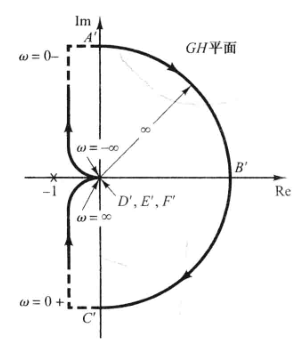
\includegraphics[width=8cm]{figures/28.png}
    \caption{$G(s)H(s)$平面上的封闭曲线}
    \label{28}
\end{figure}

\subsection{相对稳定性分析}

为了表示稳定系统的稳定程度,可以定义一系列相对稳定性参数。

\textbf{相位裕量}

开环传递函数的幅值$|G(j\omega)|$等于1时,此处的相角$\Phi$加$180^\circ$即为相位裕量

\begin{equation*}
    \gamma=180^\circ + \Phi\quad\mbox{Phase Margin, }M_f
\end{equation*}

\textbf{增益裕量}

在相角等于$-180^\circ$的频率上,幅值$|G(j\omega)|$的倒数称为增益裕量

\begin{equation*}
    K_g=\frac{1}{|G(j\omega)|}
\end{equation*}

一般以分贝表示

\begin{equation*}
    K_g(dB)=20\log K_g=-20\log |G(j\omega)|\quad\mbox{Gain Margin, }M_g
\end{equation*}

\textbf{灵敏度峰值}

以$-1,j0$为圆心,与Nyquist轨迹不相交的最大的圆的半径的倒数。

\begin{equation*}
    \frac{1}{\eta}=\frac{1}{\min|1+\Lambda_0(j\omega)|}\quad\mbox{Sensitivity Peak}
\end{equation*}

图\ref{29}展示了相对稳定性参数在伯德图和奈奎斯特图中的意义。

\begin{figure}[!ht]
    \centering
    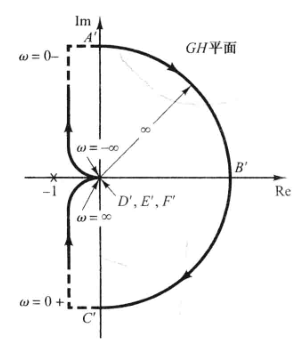
\includegraphics[width=8cm]{figures/29.png}
    \caption{相位裕量和增益裕量}
    \label{29}
\end{figure}